\section{The Finite State Machine}
The FSM is the crux of interacting with the CAPP and making it carry out complex arbitrary algorithms by exposing commands to carry out different tasks. 
It has numerous states, some of them are sending or receiving data, loading data into the CAPP, selecting first, searching, reading, setting the comparand and mask as well as writing. 
The base UART module used is from David Things' Github repository. \cite{uart} This works on a 48MHz clock cycle.
To reduce complexities and avoid additional LUTs usage, we used the same clock speed throughout the project. 
\\\\
As shown in figure 4 (TODO), our FSM acts as a way to carry out procedural tasks while staying under the limit of 21 ns by linking states together. 
Therefore, a task may trigger several states before it returns to the default state. 
For example, the algorithm for searching has several steps, it comprises of
\begin{itemize}
    \item Setting the comparand 
    \item Setting the mask 
    \item Sending the SET signal
    \item Sending the SEARCH signal 
\end{itemize}

Notice that the first two steps use several clock cycles as only one byte of data flows through the UART each clock cycle. 
This is due to its pipeline design. 
\\\\
The states transitions for the SET signal is given below:
\begin{itemize}
    \item  SET 1: change SET to high, set delay to 5 clock cycles
    \item  IDLE: wait for delay, go to SET 0
    \item  SET 0: change SET to low, listen for new command
\end{itemize}
\vspace{5mm}
This is similar to the SEARCH signal:
\begin{itemize}
    \item  SEARCH 1: change SEARCH to high, set delay to 5 clock cycles
    \item  IDLE: wait for delay, go to SEARCH 0
    \item  SEARCH 0: change SEARCH to low, listen for new command
\end{itemize}
\vspace{5mm}
The tasks that involve transmitting follow a similar state transition procedure. 
Here, a state send one character to the host through the uart each clock cycle. 
Examples of these are sending comparand, tags and mask. 
The state transition diagram of sending the comparand is shown in Figure 3.
The procedures for the other commands are similar in the way that different states just change the value of a register. 
The send state just transmits data from this register. 
This design decision was made to reduce the memory as well as number of combinatorial circuits. 

\begin{itemize}
    \item  GET COMPARAND: set output text equat to comparand
    \item  SEND: Send the next character until EOL. Listen for next command
\end{itemize}

\begin{figure}[h]
   
    \tikzset{every picture/.style={line width=0.75pt}} %set default line width to 0.75pt        

    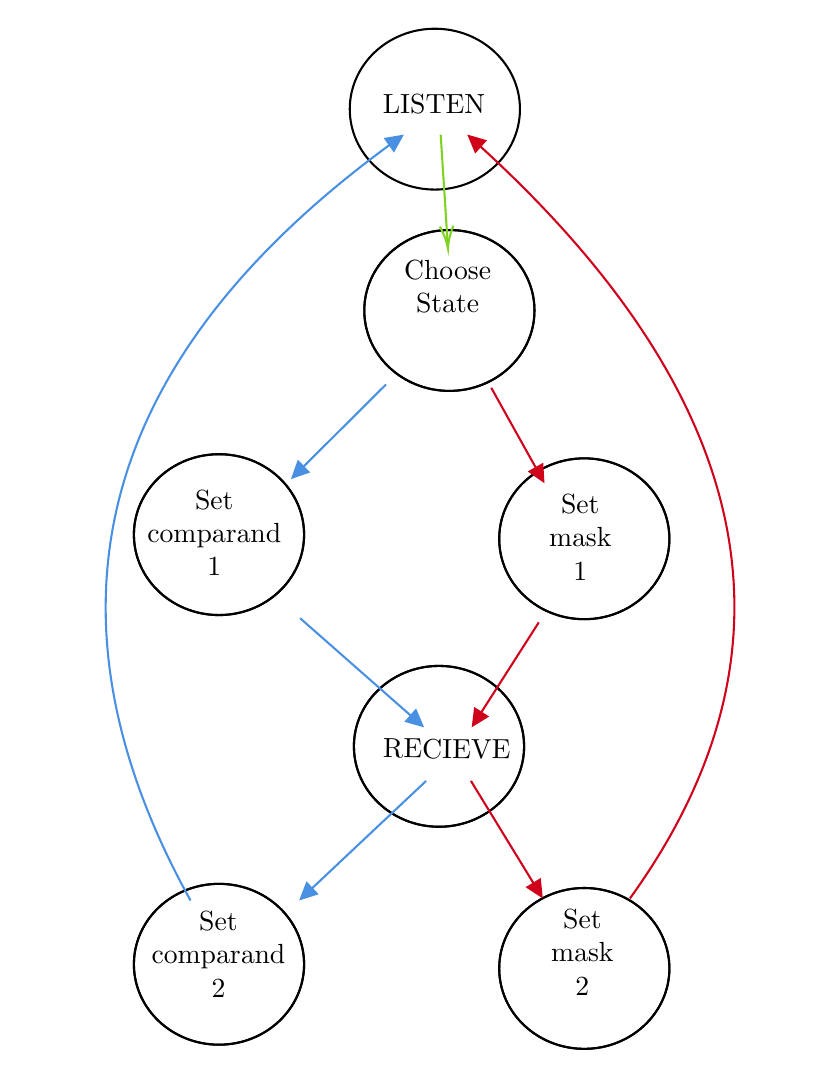
\begin{tikzpicture}[x=0.75pt,y=0.75pt,yscale=-1,xscale=1]
    %uncomment if require: \path (0,560); %set diagram left start at 0, and has height of 560

    %Shape: Ellipse [id:dp30119061586837703] 
    \draw   (123.23,354.75) .. controls (123.23,333.35) and (141.59,316) .. (164.23,316) .. controls (186.87,316) and (205.23,333.35) .. (205.23,354.75) .. controls (205.23,376.15) and (186.87,393.5) .. (164.23,393.5) .. controls (141.59,393.5) and (123.23,376.15) .. (123.23,354.75) -- cycle ;
    %Shape: Ellipse [id:dp4848885797268667] 
    \draw   (123.23,354.75) .. controls (123.23,333.35) and (141.59,316) .. (164.23,316) .. controls (186.87,316) and (205.23,333.35) .. (205.23,354.75) .. controls (205.23,376.15) and (186.87,393.5) .. (164.23,393.5) .. controls (141.59,393.5) and (123.23,376.15) .. (123.23,354.75) -- cycle ;
    %Shape: Ellipse [id:dp6948847640403879] 
    \draw   (17.23,252.75) .. controls (17.23,231.35) and (35.59,214) .. (58.23,214) .. controls (80.87,214) and (99.23,231.35) .. (99.23,252.75) .. controls (99.23,274.15) and (80.87,291.5) .. (58.23,291.5) .. controls (35.59,291.5) and (17.23,274.15) .. (17.23,252.75) -- cycle ;
    %Shape: Ellipse [id:dp2567147302347228] 
    \draw   (17.23,252.75) .. controls (17.23,231.35) and (35.59,214) .. (58.23,214) .. controls (80.87,214) and (99.23,231.35) .. (99.23,252.75) .. controls (99.23,274.15) and (80.87,291.5) .. (58.23,291.5) .. controls (35.59,291.5) and (17.23,274.15) .. (17.23,252.75) -- cycle ;
    %Shape: Ellipse [id:dp938096594364014] 
    \draw   (17.23,459.75) .. controls (17.23,438.35) and (35.59,421) .. (58.23,421) .. controls (80.87,421) and (99.23,438.35) .. (99.23,459.75) .. controls (99.23,481.15) and (80.87,498.5) .. (58.23,498.5) .. controls (35.59,498.5) and (17.23,481.15) .. (17.23,459.75) -- cycle ;
    %Shape: Ellipse [id:dp887993685343583] 
    \draw   (17.23,459.75) .. controls (17.23,438.35) and (35.59,421) .. (58.23,421) .. controls (80.87,421) and (99.23,438.35) .. (99.23,459.75) .. controls (99.23,481.15) and (80.87,498.5) .. (58.23,498.5) .. controls (35.59,498.5) and (17.23,481.15) .. (17.23,459.75) -- cycle ;
    %Shape: Ellipse [id:dp8591576771955458] 
    \draw   (128.23,144.75) .. controls (128.23,123.35) and (146.59,106) .. (169.23,106) .. controls (191.87,106) and (210.23,123.35) .. (210.23,144.75) .. controls (210.23,166.15) and (191.87,183.5) .. (169.23,183.5) .. controls (146.59,183.5) and (128.23,166.15) .. (128.23,144.75) -- cycle ;
    %Shape: Ellipse [id:dp42179166865495454] 
    \draw   (128.23,144.75) .. controls (128.23,123.35) and (146.59,106) .. (169.23,106) .. controls (191.87,106) and (210.23,123.35) .. (210.23,144.75) .. controls (210.23,166.15) and (191.87,183.5) .. (169.23,183.5) .. controls (146.59,183.5) and (128.23,166.15) .. (128.23,144.75) -- cycle ;
    %Shape: Path Data [id:dp8046463405438573] 
    \draw   (162.23,9) .. controls (184.87,9) and (203.23,26.35) .. (203.23,47.75) .. controls (203.23,69.15) and (184.87,86.5) .. (162.23,86.5) .. controls (139.59,86.5) and (121.23,69.15) .. (121.23,47.75) .. controls (121.23,26.35) and (139.59,9) .. (162.23,9) -- cycle ;
    %Shape: Ellipse [id:dp8077670693031269] 
    \draw   (193.23,254.75) .. controls (193.23,233.35) and (211.59,216) .. (234.23,216) .. controls (256.87,216) and (275.23,233.35) .. (275.23,254.75) .. controls (275.23,276.15) and (256.87,293.5) .. (234.23,293.5) .. controls (211.59,293.5) and (193.23,276.15) .. (193.23,254.75) -- cycle ;
    %Shape: Ellipse [id:dp29590588232724735] 
    \draw   (193.23,254.75) .. controls (193.23,233.35) and (211.59,216) .. (234.23,216) .. controls (256.87,216) and (275.23,233.35) .. (275.23,254.75) .. controls (275.23,276.15) and (256.87,293.5) .. (234.23,293.5) .. controls (211.59,293.5) and (193.23,276.15) .. (193.23,254.75) -- cycle ;
    %Shape: Ellipse [id:dp11804790571034007] 
    \draw   (193.23,461.75) .. controls (193.23,440.35) and (211.59,423) .. (234.23,423) .. controls (256.87,423) and (275.23,440.35) .. (275.23,461.75) .. controls (275.23,483.15) and (256.87,500.5) .. (234.23,500.5) .. controls (211.59,500.5) and (193.23,483.15) .. (193.23,461.75) -- cycle ;
    %Shape: Ellipse [id:dp29705692546094364] 
    \draw   (193.23,461.75) .. controls (193.23,440.35) and (211.59,423) .. (234.23,423) .. controls (256.87,423) and (275.23,440.35) .. (275.23,461.75) .. controls (275.23,483.15) and (256.87,500.5) .. (234.23,500.5) .. controls (211.59,500.5) and (193.23,483.15) .. (193.23,461.75) -- cycle ;

    % Text Node
    \draw (135.83,349.61) node [anchor=north west][inner sep=0.75pt]  [rotate=-0.67] [align=left] {RECIEVE};
    % Text Node
    \draw (16.73,230.01) node [anchor=north west][inner sep=0.75pt]   [align=left] {\begin{minipage}[lt]{56.588784000000004pt}\setlength\topsep{0pt}
    \begin{center}
    Set \\comparand \\1
    \end{center}

    \end{minipage}};
    % Text Node
    \draw (18.73,433.01) node [anchor=north west][inner sep=0.75pt]   [align=left] {\begin{minipage}[lt]{56.588784000000004pt}\setlength\topsep{0pt}
    \begin{center}
    Set \\comparand \\2
    \end{center}

    \end{minipage}};
    % Text Node
    \draw (139.73,119.01) node [anchor=north west][inner sep=0.75pt]   [align=left] {\begin{minipage}[lt]{40.715pt}\setlength\topsep{0pt}
    \begin{center}
    Choose \\State\\
    \end{center}

    \end{minipage}};
    % Text Node
    \draw (134.73,39.01) node [anchor=north west][inner sep=0.75pt]   [align=left] {\begin{minipage}[lt]{38.430608pt}\setlength\topsep{0pt}
    \begin{center}
    LISTEN
    \end{center}

    \end{minipage}};
    % Text Node
    \draw (212.73,232.01) node [anchor=north west][inner sep=0.75pt]   [align=left] {\begin{minipage}[lt]{27.093784000000003pt}\setlength\topsep{0pt}
    \begin{center}
    Set \\mask\\1
    \end{center}

    \end{minipage}};
    % Text Node
    \draw (213.73,432.01) node [anchor=north west][inner sep=0.75pt]   [align=left] {\begin{minipage}[lt]{27.093784000000003pt}\setlength\topsep{0pt}
    \begin{center}
    Set \\mask\\2
    \end{center}

    \end{minipage}};
    % Connection
    \draw [color={rgb, 255:red, 126; green, 211; blue, 33 }  ,draw opacity=1 ]   (165.03,60.01) -- (168.44,113.01) ;
    \draw [shift={(168.57,115.01)}, rotate = 266.32] [color={rgb, 255:red, 126; green, 211; blue, 33 }  ,draw opacity=1 ][line width=0.75]    (10.93,-3.29) .. controls (6.95,-1.4) and (3.31,-0.3) .. (0,0) .. controls (3.31,0.3) and (6.95,1.4) .. (10.93,3.29)   ;
    % Connection
    \draw [color={rgb, 255:red, 74; green, 144; blue, 226 }  ,draw opacity=1 ]   (138.73,180.37) -- (95.01,223.89) ;
    \draw [shift={(92.88,226.01)}, rotate = 315.13] [fill={rgb, 255:red, 74; green, 144; blue, 226 }  ,fill opacity=1 ][line width=0.08]  [draw opacity=0] (8.93,-4.29) -- (0,0) -- (8.93,4.29) -- cycle    ;
    % Connection
    \draw [color={rgb, 255:red, 74; green, 144; blue, 226 }  ,draw opacity=1 ]   (97.3,293.01) -- (154.81,343.62) ;
    \draw [shift={(157.06,345.6)}, rotate = 221.35] [fill={rgb, 255:red, 74; green, 144; blue, 226 }  ,fill opacity=1 ][line width=0.08]  [draw opacity=0] (8.93,-4.29) -- (0,0) -- (8.93,4.29) -- cycle    ;
    % Connection
    \draw [color={rgb, 255:red, 74; green, 144; blue, 226 }  ,draw opacity=1 ]   (158.01,371.42) -- (99.01,426.95) ;
    \draw [shift={(96.82,429.01)}, rotate = 316.74] [fill={rgb, 255:red, 74; green, 144; blue, 226 }  ,fill opacity=1 ][line width=0.08]  [draw opacity=0] (8.93,-4.29) -- (0,0) -- (8.93,4.29) -- cycle    ;
    % Connection
    \draw [color={rgb, 255:red, 208; green, 2; blue, 27 }  ,draw opacity=1 ]   (189.41,182.01) -- (213.59,225.39) ;
    \draw [shift={(215.05,228.01)}, rotate = 240.86] [fill={rgb, 255:red, 208; green, 2; blue, 27 }  ,fill opacity=1 ][line width=0.08]  [draw opacity=0] (8.93,-4.29) -- (0,0) -- (8.93,4.29) -- cycle    ;
    % Connection
    \draw [color={rgb, 255:red, 208; green, 2; blue, 27 }  ,draw opacity=1 ]   (256.24,428.01) .. controls (342.98,307.61) and (317.55,185.57) .. (179.92,61.87) ;
    \draw [shift={(177.84,60.01)}, rotate = 401.72] [fill={rgb, 255:red, 208; green, 2; blue, 27 }  ,fill opacity=1 ][line width=0.08]  [draw opacity=0] (8.93,-4.29) -- (0,0) -- (8.93,4.29) -- cycle    ;
    % Connection
    \draw [color={rgb, 255:red, 74; green, 144; blue, 226 }  ,draw opacity=1 ]   (44.51,429.01) .. controls (-33.45,288.05) and (0.1,165.57) .. (145.13,61.58) ;
    \draw [shift={(147.33,60.01)}, rotate = 504.61] [fill={rgb, 255:red, 74; green, 144; blue, 226 }  ,fill opacity=1 ][line width=0.08]  [draw opacity=0] (8.93,-4.29) -- (0,0) -- (8.93,4.29) -- cycle    ;
    % Connection
    \draw [color={rgb, 255:red, 208; green, 2; blue, 27 }  ,draw opacity=1 ]   (212.32,295.01) -- (181.6,343.07) ;
    \draw [shift={(179.98,345.6)}, rotate = 302.59000000000003] [fill={rgb, 255:red, 208; green, 2; blue, 27 }  ,fill opacity=1 ][line width=0.08]  [draw opacity=0] (8.93,-4.29) -- (0,0) -- (8.93,4.29) -- cycle    ;
    % Connection
    \draw [color={rgb, 255:red, 208; green, 2; blue, 27 }  ,draw opacity=1 ]   (179.62,371.42) -- (212.67,425.45) ;
    \draw [shift={(214.24,428.01)}, rotate = 238.55] [fill={rgb, 255:red, 208; green, 2; blue, 27 }  ,fill opacity=1 ][line width=0.08]  [draw opacity=0] (8.93,-4.29) -- (0,0) -- (8.93,4.29) -- cycle    ;

    \end{tikzpicture}
    \caption{The transitions of the FSM for setting the comparand (blue) and the mask (red). Each transition happens on a different clock cycle to maintain the inner state of the memory and to allow time for the data to complete its flow. }
\end{figure}
    
\begin{figure}
\tikzset{every picture/.style={line width=0.75pt}} %set default line width to 0.75pt        

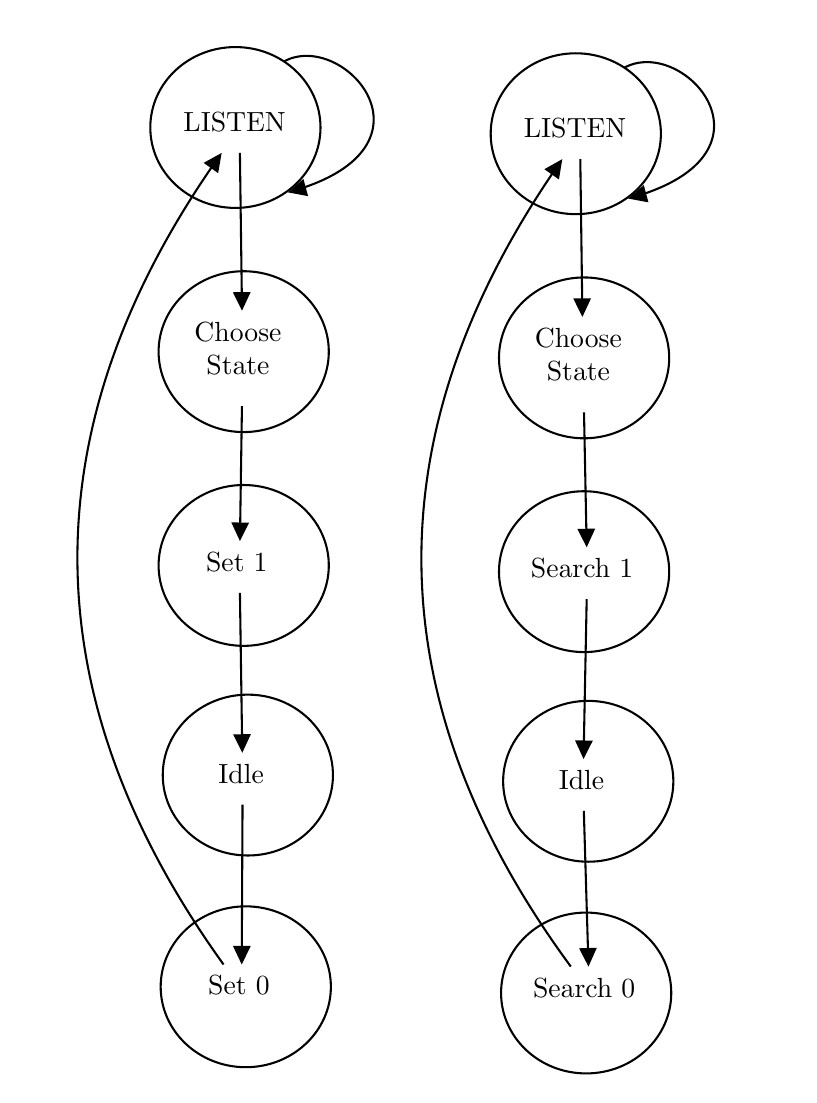
\begin{tikzpicture}[x=0.75pt,y=0.75pt,yscale=-1,xscale=1]
%uncomment if require: \path (0,560); %set diagram left start at 0, and has height of 560

%Shape: Path Data [id:dp8046463405438573] 
\draw   (78.23,5) .. controls (100.87,5) and (119.23,22.35) .. (119.23,43.75) .. controls (119.23,65.15) and (100.87,82.5) .. (78.23,82.5) .. controls (55.59,82.5) and (37.23,65.15) .. (37.23,43.75) .. controls (37.23,22.35) and (55.59,5) .. (78.23,5) -- cycle ;
%Shape: Path Data [id:dp8728363006705233] 
\draw   (82.23,113) .. controls (104.87,113) and (123.23,130.35) .. (123.23,151.75) .. controls (123.23,173.15) and (104.87,190.5) .. (82.23,190.5) .. controls (59.59,190.5) and (41.23,173.15) .. (41.23,151.75) .. controls (41.23,130.35) and (59.59,113) .. (82.23,113) -- cycle ;
%Shape: Path Data [id:dp7565150984427305] 
\draw   (82.23,216) .. controls (104.87,216) and (123.23,233.35) .. (123.23,254.75) .. controls (123.23,276.15) and (104.87,293.5) .. (82.23,293.5) .. controls (59.59,293.5) and (41.23,276.15) .. (41.23,254.75) .. controls (41.23,233.35) and (59.59,216) .. (82.23,216) -- cycle ;
%Shape: Path Data [id:dp2088156148286131] 
\draw   (84.23,317) .. controls (106.87,317) and (125.23,334.35) .. (125.23,355.75) .. controls (125.23,377.15) and (106.87,394.5) .. (84.23,394.5) .. controls (61.59,394.5) and (43.23,377.15) .. (43.23,355.75) .. controls (43.23,334.35) and (61.59,317) .. (84.23,317) -- cycle ;
%Shape: Path Data [id:dp49675905995877145] 
\draw   (83.23,419) .. controls (105.87,419) and (124.23,436.35) .. (124.23,457.75) .. controls (124.23,479.15) and (105.87,496.5) .. (83.23,496.5) .. controls (60.59,496.5) and (42.23,479.15) .. (42.23,457.75) .. controls (42.23,436.35) and (60.59,419) .. (83.23,419) -- cycle ;
%Curve Lines [id:da7232392383634552] 
\draw    (101.5,12) .. controls (130.21,-3.84) and (180.48,52.85) .. (105.8,74.36) ;
\draw [shift={(103.5,75)}, rotate = 344.93] [fill={rgb, 255:red, 0; green, 0; blue, 0 }  ][line width=0.08]  [draw opacity=0] (8.93,-4.29) -- (0,0) -- (8.93,4.29) -- cycle    ;
%Shape: Path Data [id:dp4471286129350249] 
\draw   (242.23,8) .. controls (264.87,8) and (283.23,25.35) .. (283.23,46.75) .. controls (283.23,68.15) and (264.87,85.5) .. (242.23,85.5) .. controls (219.59,85.5) and (201.23,68.15) .. (201.23,46.75) .. controls (201.23,25.35) and (219.59,8) .. (242.23,8) -- cycle ;
%Shape: Path Data [id:dp29112909354894145] 
\draw   (246.23,116) .. controls (268.87,116) and (287.23,133.35) .. (287.23,154.75) .. controls (287.23,176.15) and (268.87,193.5) .. (246.23,193.5) .. controls (223.59,193.5) and (205.23,176.15) .. (205.23,154.75) .. controls (205.23,133.35) and (223.59,116) .. (246.23,116) -- cycle ;
%Shape: Path Data [id:dp19350350344214817] 
\draw   (246.23,219) .. controls (268.87,219) and (287.23,236.35) .. (287.23,257.75) .. controls (287.23,279.15) and (268.87,296.5) .. (246.23,296.5) .. controls (223.59,296.5) and (205.23,279.15) .. (205.23,257.75) .. controls (205.23,236.35) and (223.59,219) .. (246.23,219) -- cycle ;
%Shape: Path Data [id:dp41437519393069566] 
\draw   (248.23,320) .. controls (270.87,320) and (289.23,337.35) .. (289.23,358.75) .. controls (289.23,380.15) and (270.87,397.5) .. (248.23,397.5) .. controls (225.59,397.5) and (207.23,380.15) .. (207.23,358.75) .. controls (207.23,337.35) and (225.59,320) .. (248.23,320) -- cycle ;
%Shape: Path Data [id:dp5957992985412117] 
\draw   (247.23,422) .. controls (269.87,422) and (288.23,439.35) .. (288.23,460.75) .. controls (288.23,482.15) and (269.87,499.5) .. (247.23,499.5) .. controls (224.59,499.5) and (206.23,482.15) .. (206.23,460.75) .. controls (206.23,439.35) and (224.59,422) .. (247.23,422) -- cycle ;
%Curve Lines [id:da08134101622369627] 
\draw    (265.5,15) .. controls (294.21,-0.84) and (344.48,55.85) .. (269.8,77.36) ;
\draw [shift={(267.5,78)}, rotate = 344.93] [fill={rgb, 255:red, 0; green, 0; blue, 0 }  ][line width=0.08]  [draw opacity=0] (8.93,-4.29) -- (0,0) -- (8.93,4.29) -- cycle    ;

% Text Node
\draw (50.73,35.01) node [anchor=north west][inner sep=0.75pt]   [align=left] {\begin{minipage}[lt]{38.430608pt}\setlength\topsep{0pt}
\begin{center}
LISTEN
\end{center}

\end{minipage}};
% Text Node
\draw (52.73,136.01) node [anchor=north west][inner sep=0.75pt]   [align=left] {\begin{minipage}[lt]{37.878108000000005pt}\setlength\topsep{0pt}
\begin{center}
Choose\\ State
\end{center}

\end{minipage}};
% Text Node
\draw (59.73,247.01) node [anchor=north west][inner sep=0.75pt]   [align=left] {\begin{minipage}[lt]{26.541216000000002pt}\setlength\topsep{0pt}
\begin{center}
Set 1
\end{center}

\end{minipage}};
% Text Node
\draw (66.73,349.01) node [anchor=north west][inner sep=0.75pt]   [align=left] {\begin{minipage}[lt]{19.1675pt}\setlength\topsep{0pt}
\begin{center}
Idle
\end{center}

\end{minipage}};
% Text Node
\draw (60.73,451.01) node [anchor=north west][inner sep=0.75pt]   [align=left] {\begin{minipage}[lt]{26.541216000000002pt}\setlength\topsep{0pt}
\begin{center}
Set 0
\end{center}

\end{minipage}};
% Text Node
\draw (214.73,38.01) node [anchor=north west][inner sep=0.75pt]   [align=left] {\begin{minipage}[lt]{38.430608pt}\setlength\topsep{0pt}
\begin{center}
LISTEN
\end{center}

\end{minipage}};
% Text Node
\draw (216.73,139.01) node [anchor=north west][inner sep=0.75pt]   [align=left] {\begin{minipage}[lt]{37.878108000000005pt}\setlength\topsep{0pt}
\begin{center}
Choose\\ State
\end{center}

\end{minipage}};
% Text Node
\draw (214.73,250.01) node [anchor=north west][inner sep=0.75pt]   [align=left] {\begin{minipage}[lt]{43.551892pt}\setlength\topsep{0pt}
\begin{center}
Search 1
\end{center}

\end{minipage}};
% Text Node
\draw (230.73,352.01) node [anchor=north west][inner sep=0.75pt]   [align=left] {\begin{minipage}[lt]{19.1675pt}\setlength\topsep{0pt}
\begin{center}
Idle
\end{center}

\end{minipage}};
% Text Node
\draw (215.73,452.01) node [anchor=north west][inner sep=0.75pt]   [align=left] {\begin{minipage}[lt]{43.551892pt}\setlength\topsep{0pt}
\begin{center}
Search 0
\end{center}

\end{minipage}};
% Connection
\draw [color={rgb, 255:red, 0; green, 0; blue, 0 }  ,draw opacity=1 ]   (80.4,56.01) -- (81.38,129.01) ;
\draw [shift={(81.42,132.01)}, rotate = 269.23] [fill={rgb, 255:red, 0; green, 0; blue, 0 }  ,fill opacity=1 ][line width=0.08]  [draw opacity=0] (8.93,-4.29) -- (0,0) -- (8.93,4.29) -- cycle    ;
% Connection
\draw    (81.39,178.01) -- (80.46,240.01) ;
\draw [shift={(80.42,243.01)}, rotate = 270.86] [fill={rgb, 255:red, 0; green, 0; blue, 0 }  ][line width=0.08]  [draw opacity=0] (8.93,-4.29) -- (0,0) -- (8.93,4.29) -- cycle    ;
% Connection
\draw    (80.41,268.01) -- (81.5,342.01) ;
\draw [shift={(81.54,345.01)}, rotate = 269.15999999999997] [fill={rgb, 255:red, 0; green, 0; blue, 0 }  ][line width=0.08]  [draw opacity=0] (8.93,-4.29) -- (0,0) -- (8.93,4.29) -- cycle    ;
% Connection
\draw    (81.67,370.01) -- (81.3,444.01) ;
\draw [shift={(81.29,447.01)}, rotate = 270.28] [fill={rgb, 255:red, 0; green, 0; blue, 0 }  ][line width=0.08]  [draw opacity=0] (8.93,-4.29) -- (0,0) -- (8.93,4.29) -- cycle    ;
% Connection
\draw    (72.52,447.01) .. controls (-20.59,317.57) and (-21.35,187.88) .. (70.22,57.97) ;
\draw [shift={(71.61,56.01)}, rotate = 485.45] [fill={rgb, 255:red, 0; green, 0; blue, 0 }  ][line width=0.08]  [draw opacity=0] (8.93,-4.29) -- (0,0) -- (8.93,4.29) -- cycle    ;
% Connection
\draw [color={rgb, 255:red, 0; green, 0; blue, 0 }  ,draw opacity=1 ]   (244.4,59.01) -- (245.38,132.01) ;
\draw [shift={(245.42,135.01)}, rotate = 269.23] [fill={rgb, 255:red, 0; green, 0; blue, 0 }  ,fill opacity=1 ][line width=0.08]  [draw opacity=0] (8.93,-4.29) -- (0,0) -- (8.93,4.29) -- cycle    ;
% Connection
\draw    (246.19,181.01) -- (247.42,243.01) ;
\draw [shift={(247.48,246.01)}, rotate = 268.86] [fill={rgb, 255:red, 0; green, 0; blue, 0 }  ][line width=0.08]  [draw opacity=0] (8.93,-4.29) -- (0,0) -- (8.93,4.29) -- cycle    ;
% Connection
\draw    (247.48,271.01) -- (246.03,345.01) ;
\draw [shift={(245.97,348.01)}, rotate = 271.12] [fill={rgb, 255:red, 0; green, 0; blue, 0 }  ][line width=0.08]  [draw opacity=0] (8.93,-4.29) -- (0,0) -- (8.93,4.29) -- cycle    ;
% Connection
\draw    (246.1,373.01) -- (248.26,445.01) ;
\draw [shift={(248.35,448.01)}, rotate = 268.28] [fill={rgb, 255:red, 0; green, 0; blue, 0 }  ][line width=0.08]  [draw opacity=0] (8.93,-4.29) -- (0,0) -- (8.93,4.29) -- cycle    ;
% Connection
\draw    (239.83,448.01) .. controls (145.7,320.06) and (143.88,191.05) .. (234.36,60.97) ;
\draw [shift={(235.73,59.01)}, rotate = 485.09] [fill={rgb, 255:red, 0; green, 0; blue, 0 }  ][line width=0.08]  [draw opacity=0] (8.93,-4.29) -- (0,0) -- (8.93,4.29) -- cycle    ;

\end{tikzpicture}
\caption{The transitions of the FSM for (left) sending signals for seeting all tag bits high, as well as (right) performing search using the comparand and the mask.}

\end{figure}

\begin{figure}
    

\tikzset{every picture/.style={line width=0.75pt}} %set default line width to 0.75pt        

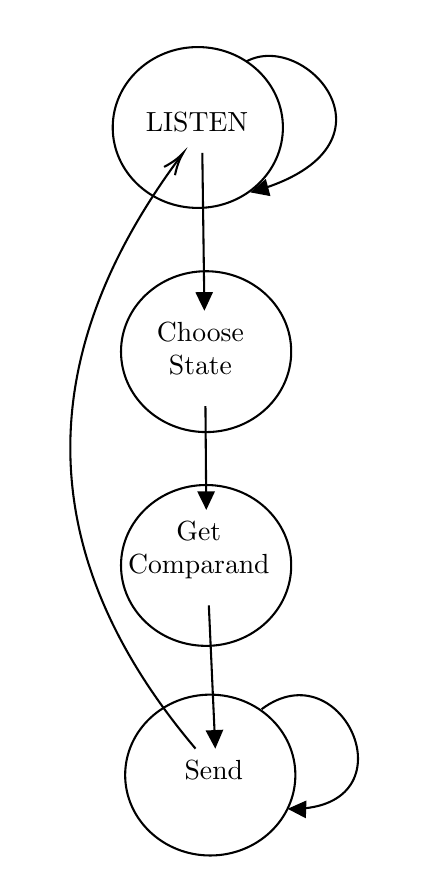
\begin{tikzpicture}[x=0.75pt,y=0.75pt,yscale=-1,xscale=1]
%uncomment if require: \path (0,560); %set diagram left start at 0, and has height of 560

%Shape: Path Data [id:dp8046463405438573] 
\draw   (78.23,5) .. controls (100.87,5) and (119.23,22.35) .. (119.23,43.75) .. controls (119.23,65.15) and (100.87,82.5) .. (78.23,82.5) .. controls (55.59,82.5) and (37.23,65.15) .. (37.23,43.75) .. controls (37.23,22.35) and (55.59,5) .. (78.23,5) -- cycle ;
%Shape: Path Data [id:dp8728363006705233] 
\draw   (82.23,113) .. controls (104.87,113) and (123.23,130.35) .. (123.23,151.75) .. controls (123.23,173.15) and (104.87,190.5) .. (82.23,190.5) .. controls (59.59,190.5) and (41.23,173.15) .. (41.23,151.75) .. controls (41.23,130.35) and (59.59,113) .. (82.23,113) -- cycle ;
%Shape: Path Data [id:dp7565150984427305] 
\draw   (82.23,216) .. controls (104.87,216) and (123.23,233.35) .. (123.23,254.75) .. controls (123.23,276.15) and (104.87,293.5) .. (82.23,293.5) .. controls (59.59,293.5) and (41.23,276.15) .. (41.23,254.75) .. controls (41.23,233.35) and (59.59,216) .. (82.23,216) -- cycle ;
%Shape: Path Data [id:dp2088156148286131] 
\draw   (84.23,317) .. controls (106.87,317) and (125.23,334.35) .. (125.23,355.75) .. controls (125.23,377.15) and (106.87,394.5) .. (84.23,394.5) .. controls (61.59,394.5) and (43.23,377.15) .. (43.23,355.75) .. controls (43.23,334.35) and (61.59,317) .. (84.23,317) -- cycle ;
%Curve Lines [id:da7232392383634552] 
\draw    (101.5,12) .. controls (130.21,-3.84) and (180.48,52.85) .. (105.8,74.36) ;
\draw [shift={(103.5,75)}, rotate = 344.93] [fill={rgb, 255:red, 0; green, 0; blue, 0 }  ][line width=0.08]  [draw opacity=0] (8.93,-4.29) -- (0,0) -- (8.93,4.29) -- cycle    ;
%Curve Lines [id:da7972995956061577] 
\draw    (109,324) .. controls (148.4,294.45) and (182.46,371.62) .. (124.23,372.04) ;
\draw [shift={(121.5,372)}, rotate = 361.85] [fill={rgb, 255:red, 0; green, 0; blue, 0 }  ][line width=0.08]  [draw opacity=0] (8.93,-4.29) -- (0,0) -- (8.93,4.29) -- cycle    ;

% Text Node
\draw (50.73,35.01) node [anchor=north west][inner sep=0.75pt]   [align=left] {\begin{minipage}[lt]{38.430608pt}\setlength\topsep{0pt}
\begin{center}
LISTEN
\end{center}

\end{minipage}};
% Text Node
\draw (52.73,136.01) node [anchor=north west][inner sep=0.75pt]   [align=left] {\begin{minipage}[lt]{37.878108000000005pt}\setlength\topsep{0pt}
\begin{center}
Choose\\ State
\end{center}

\end{minipage}};
% Text Node
\draw (38,232) node [anchor=north west][inner sep=0.75pt]   [align=left] {\begin{minipage}[lt]{58.851892pt}\setlength\topsep{0pt}
\begin{center}
Get\\ Comparand
\end{center}

\end{minipage}};
% Text Node
\draw (66.73,347.01) node [anchor=north west][inner sep=0.75pt]   [align=left] {\begin{minipage}[lt]{26.551892000000002pt}\setlength\topsep{0pt}
\begin{center}
Send
\end{center}

\end{minipage}};
% Connection
\draw [color={rgb, 255:red, 0; green, 0; blue, 0 }  ,draw opacity=1 ]   (80.4,56.01) -- (81.38,129.01) ;
\draw [shift={(81.42,132.01)}, rotate = 269.23] [fill={rgb, 255:red, 0; green, 0; blue, 0 }  ,fill opacity=1 ][line width=0.08]  [draw opacity=0] (8.93,-4.29) -- (0,0) -- (8.93,4.29) -- cycle    ;
% Connection
\draw    (81.91,178.01) -- (82.29,225) ;
\draw [shift={(82.32,228)}, rotate = 269.54] [fill={rgb, 255:red, 0; green, 0; blue, 0 }  ][line width=0.08]  [draw opacity=0] (8.93,-4.29) -- (0,0) -- (8.93,4.29) -- cycle    ;
% Connection
\draw    (83.54,274) -- (86.53,340.01) ;
\draw [shift={(86.66,343.01)}, rotate = 267.40999999999997] [fill={rgb, 255:red, 0; green, 0; blue, 0 }  ][line width=0.08]  [draw opacity=0] (8.93,-4.29) -- (0,0) -- (8.93,4.29) -- cycle    ;
% Connection
\draw    (77.13,343.01) .. controls (-0.89,250.79) and (-3.24,155.62) .. (70.08,57.49) ;
\draw [shift={(71.19,56.01)}, rotate = 487.04] [color={rgb, 255:red, 0; green, 0; blue, 0 }  ][line width=0.75]    (10.93,-3.29) .. controls (6.95,-1.4) and (3.31,-0.3) .. (0,0) .. controls (3.31,0.3) and (6.95,1.4) .. (10.93,3.29)   ;

\end{tikzpicture}
\caption{State transition diagram for sending data to the host. The Get Comparand state sets output text as comparand and moves on to the Send state which transmits the data byte by byte. }
\end{figure}